\documentclass[border=10pt]{standalone}
\usepackage[svgnames]{xcolor}
\usepackage{amsmath}
\usepackage{pgfplots}
\pgfplotsset{compat=newest}
\usepackage[sfdefault]{FiraSans}
\usepackage{FiraMono}
\renewcommand*\familydefault{\sfdefault}
\begin{document}
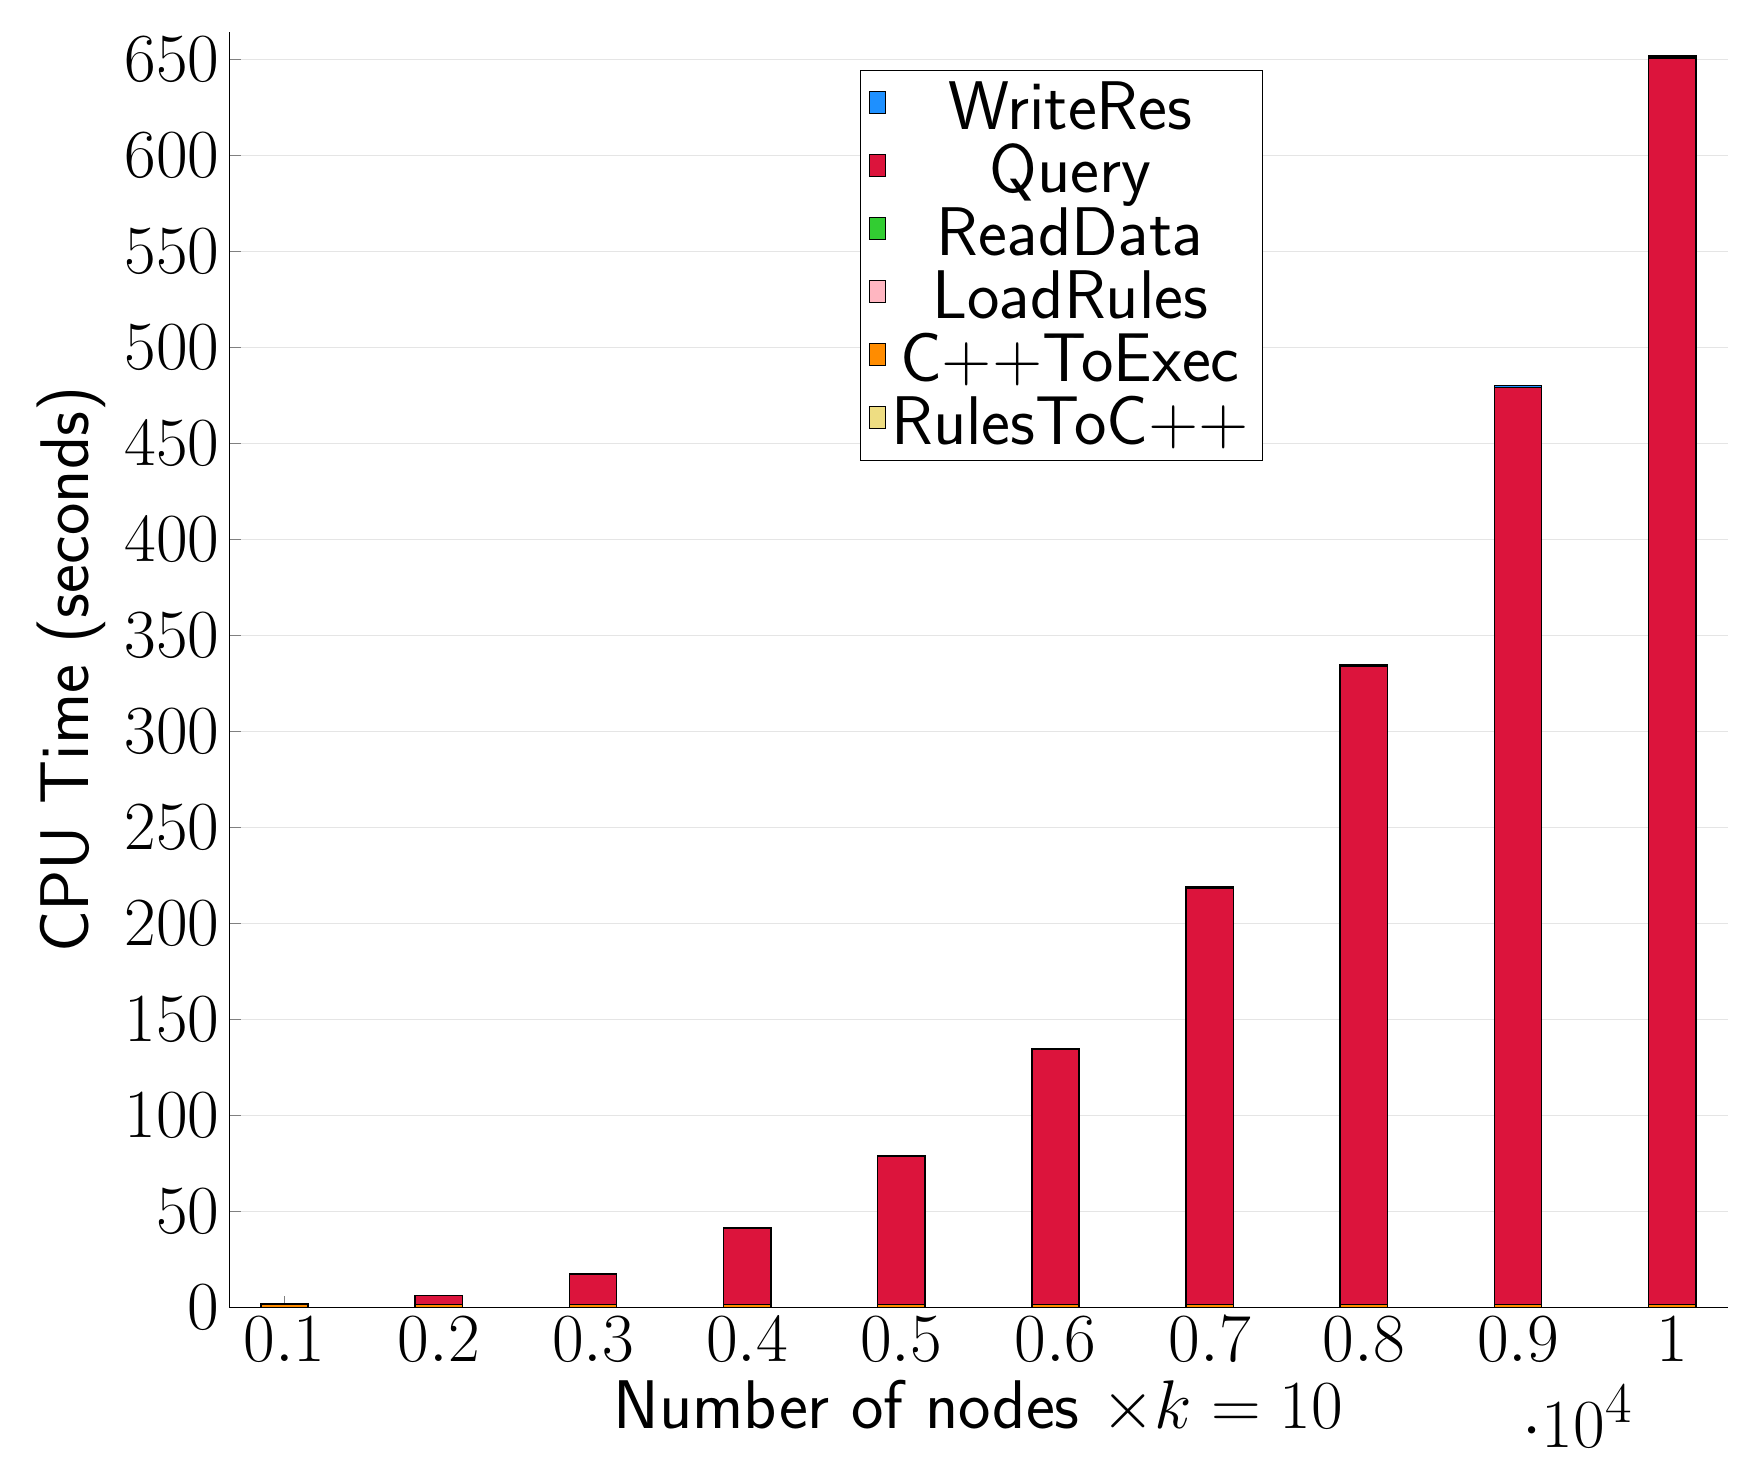
\begin{tikzpicture}
\begin{axis}[
   ybar stacked,
   width=1.7\textwidth,
   bar width=0.6cm,
   ymajorgrids, tick align=inside,
   major grid style={draw=gray!20},
   xtick=data,
   ymin=0, ymax=664.059,
   axis x line*=bottom,
   axis y line*=left,
   enlarge x limits=0.04,
   legend style={
       at={(0.69, 0.97)},
       anchor=north east,
       legend columns=1,
       font=\Huge,
   },
   ylabel={CPU Time (seconds)},
   xlabel={Number of nodes $\times k=10$},
   label style={font=\Huge},
   tick label style={font=\Huge},
]
\addlegendimage{fill=DodgerBlue, draw=black, line width=0.2pt}
\addlegendentry{WriteRes}
\addlegendimage{fill=Crimson, draw=black, line width=0.2pt}
\addlegendentry{Query}
\addlegendimage{fill=LimeGreen, draw=black, line width=0.2pt}
\addlegendentry{ReadData}
\addlegendimage{fill=LightPink, draw=black, line width=0.2pt}
\addlegendentry{LoadRules}
\addlegendimage{fill=DarkOrange, draw=black, line width=0.2pt}
\addlegendentry{C++ToExec}
\addlegendimage{fill=LightGoldenrod, draw=black, line width=0.2pt}
\addlegendentry{RulesToC++}
\addplot +[fill=LightGoldenrod, draw=black, line width=0.55pt] coordinates {
(1000, 0.004000000000000001)
(2000, 0.0020000000000000005)
(3000, 0.004000000000000001)
(4000, 0.0)
(5000, 0.0020000000000000005)
(6000, 0.0)
(7000, 0.0020000000000000005)
(8000, 0.007999999999999997)
(9000, 0.0)
(10000, 0.003999999999999997)
};
\addplot +[fill=DarkOrange, draw=black, line width=0.55pt] coordinates {
(1000, 1.4740000000000002)
(2000, 1.474)
(3000, 1.47)
(4000, 1.468)
(5000, 1.472)
(6000, 1.4779999999999998)
(7000, 1.48)
(8000, 1.476)
(9000, 1.482)
(10000, 1.4760000000000002)
};
\addplot +[fill=LightPink, draw=black, line width=0.55pt] coordinates {
(1000, 0.00018119999999999999)
(2000, 0.0001794)
(3000, 0.000196)
(4000, 0.0002058)
(5000, 0.0002204)
(6000, 0.00020119999999999998)
(7000, 0.00018020000000000002)
(8000, 0.00019260000000000002)
(9000, 0.0001938)
(10000, 0.0002056)
};
\addplot +[fill=LimeGreen, draw=black, line width=0.55pt] coordinates {
(1000, 0.004066600000000001)
(2000, 0.007144599999999999)
(3000, 0.0102306)
(4000, 0.0137874)
(5000, 0.0153112)
(6000, 0.018166)
(7000, 0.0180116)
(8000, 0.020606400000000004)
(9000, 0.022085800000000003)
(10000, 0.025811999999999995)
};
\addplot +[fill=Crimson, draw=black, line width=0.55pt] coordinates {
(1000, 0.6201072)
(2000, 4.8246780000000005)
(3000, 15.861160000000002)
(4000, 39.852419999999995)
(5000, 77.29784)
(6000, 132.69580000000002)
(7000, 216.7926)
(8000, 332.5596)
(9000, 477.6094)
(10000, 649.059)
};
\addplot +[fill=DodgerBlue, draw=black, line width=0.55pt] coordinates {
(1000, 0.0108664)
(2000, 0.0432386)
(3000, 0.09741740000000002)
(4000, 0.17434319999999998)
(5000, 0.2687214)
(6000, 0.384685)
(7000, 0.526432)
(8000, 0.6820733999999999)
(9000, 0.8626343999999999)
(10000, 1.065892)
};
\end{axis}
\end{tikzpicture}

\end{document}
